%%
%% This is file `docultex.tex', 
%% Documentation for siam macros for use with LaTeX 2e
%% 
%% August 1, 1995
%%
%% Version 1.1a
%% 
%% You are not allowed to change this file. 
%% 
%% You are allowed to distribute this file under the condition that 
%% it is distributed together with all of the files in the siam macro 
%% distribution. These are:
%%
%%  siamltex.cls (main LaTeX macro for SIAM)
%%  siamltex.sty (includes siamltex.cls for compatibility mode)
%%  siam10.clo   (size option for 10pt papers)
%%  subeqn.clo   (allows equation numbners with lettered subelements)
%%  siam.bst     (bibliographic style file for BibTeX)
%%  docultex.tex (this file)
%%  lexample.tex (example file for latex macro)
%%
%% If you receive only some of these files from someone, complain! 
%% 
%% You are NOT ALLOWED to distribute this file alone. You are NOT 
%% ALLOWED to take money for the distribution or use of either this 
%% file or a changed version, except for a nominal charge for copying 
%% etc. 
%% \CharacterTable
%%  {Upper-case    \A\B\C\D\E\F\G\H\I\J\K\L\M\N\O\P\Q\R\S\T\U\V\W\X\Y\Z
%%   Lower-case    \a\b\c\d\e\f\g\h\i\j\k\l\m\n\o\p\q\r\s\t\u\v\w\x\y\z
%%   Digits        \0\1\2\3\4\5\6\7\8\9
%%   Exclamation   \!     Double quote  \"     Hash (number) \#
%%   Dollar        \$     Percent       \%     Ampersand     \&
%%   Acute accent  \'     Left paren    \(     Right paren   \)
%%   Asterisk      \*     Plus          \+     Comma         \,
%%   Minus         \-     Point         \.     Solidus       \/
%%   Colon         \:     Semicolon     \;     Less than     \<
%%   Equals        \=     Greater than  \>     Question mark \?
%%   Commercial at \@     Left bracket  \[     Backslash     \\
%%   Right bracket \]     Circumflex    \^     Underscore    \_
%%   Grave accent  \`     Left brace    \{     Vertical bar  \|
%%   Right brace   \}     Tilde         \~}


\documentclass[final]{siamltex}

\usepackage{graphicx,float,wrapfig}


\title{Geometric Multigrid for a Jacobian-Free 
Newton Krylov Solver}

\author{William R. Boyd\thanks{Massachusetts Institute
of Technology, Nuclear Science \& Engineering, Cambridge, 
Massachusetts (wboyd@mit.edu).}}


\begin{document}
\maketitle

\begin{abstract}
The objective of this term project was to evaluate a 
Jacobian-Free Newton-Krylov (JFNK) method with multi-grid 
preconditioning.
\end{abstract}


\pagestyle{myheadings}
\thispagestyle{plain}
\markboth{TEX PRODUCTION}{USING SIAM'S \LaTeX\ MACROS}

\section{Introduction}
Hmmmmmmmm

\subsection{Hmmmm}

\section{2D LRA Benchmark Problem}
I applied my iterative solvers to the 2D LRA neutron 
diffusion problem. This benchmark problem requires
solving for the neutron flux distribution within a simplified 
quarter-core of a typical pressurized light water nuclear 
reactor. The materials in the core are considered to be 
homogeneous in 15 cm $\times$ 15 cm cells as described in 
Figure \ref{fig:materials_fine_mesh} below. The nuclear data 
used for this simple benchmark problem - including absorption, 
fission, and scattering cross-sections - are condensed from 
continuous data by a 2-group energy approximation. 
The neutron diffusion equation is solved for the flux 
distribution for each energy group.

\begin{figure}[hb!]
	\centering
	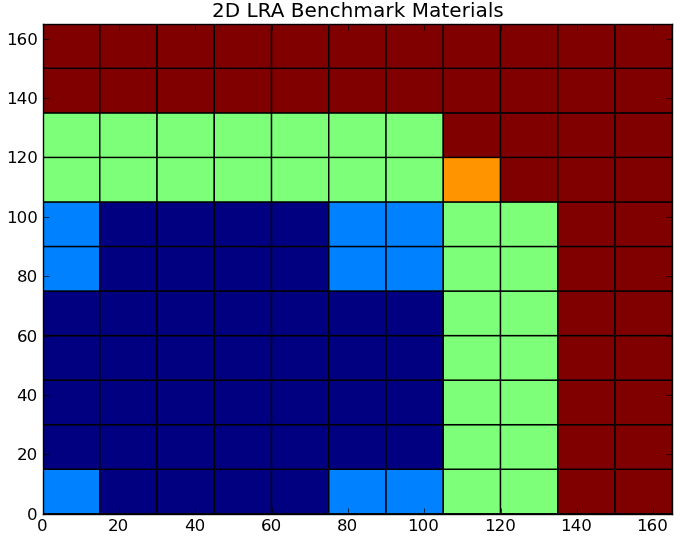
\includegraphics[scale=0.5]{materials_coarse_mesh.png}
\label{fig:materials_fine_mesh}
\caption{The coarse mesh materials design for the 2D LRA
benchmark problem. Different enrichments of UO2 fuel
are designated by dark/light blue, green and orange. Red
represents a water reflector region.}
\end{figure}

\begin{figure}[hb!]
	\centering
	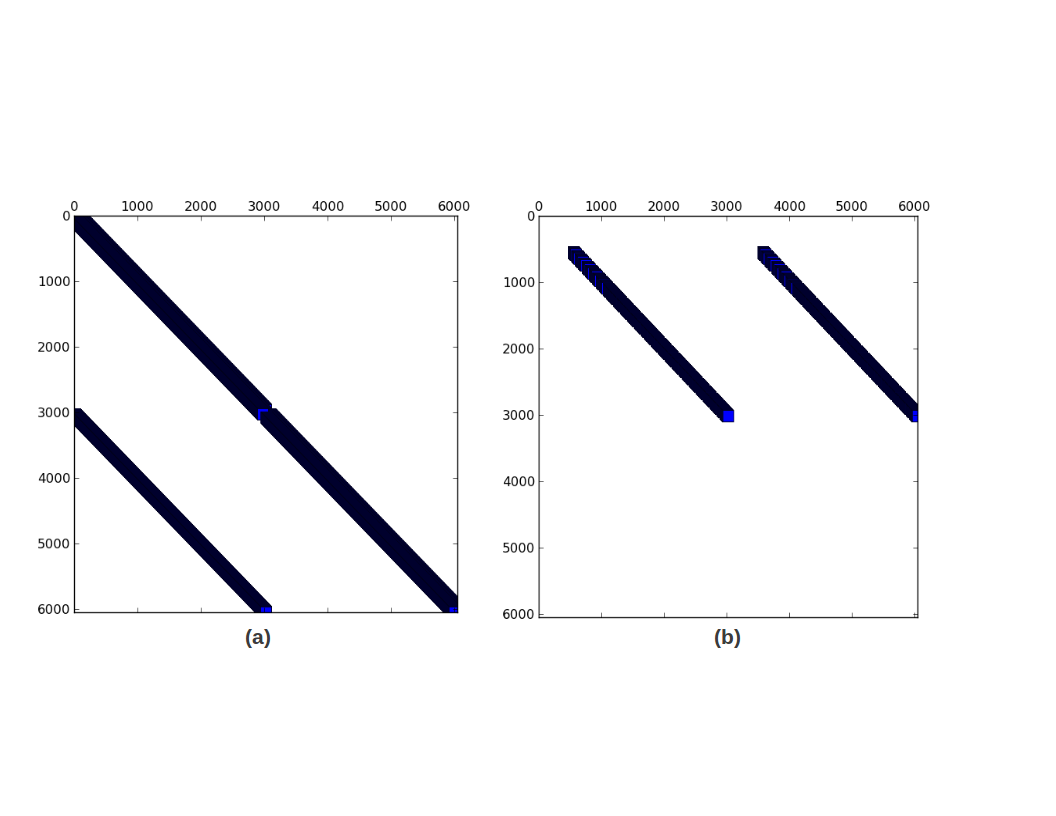
\includegraphics[scale=0.5]{M_F_full.png}
\label{fig:M_F_full}
\caption{}
\end{figure}



\section{Jacobian-Free Newton Krylov}

\section{Geometric Multi-Grid}

\section{Methodology}

\section{Results}



\begin{verbatim}

\begin{subequations}\label{EKx}
\begin{equation}
 y_k =  B  y_{k-1} +  f, \qquad k=1,2,3,\ldots  
\end{equation}
for  any initial vector $ y_0$.   Then 
\begin{equation}
 y_k\rightarrow  u \mbox{\quad iff\quad} \rho( B)<1.
\end{equation}
\end{subequations}

\end{verbatim}


\section{Bibliography and Bib\TeX}

If using {\sc Bib}\TeX, authors need not submit the {\tt .bib} file for
their papers. Merely submit the completed {\tt .bbl} file, having used
{\tt siam.bst} as their bibliographic style file. {\tt siam.bst}
only works with Bib\TeX\ version 99i and later. The use of
Bib\TeX\ and the preparation of a {\tt .bib} file is
described in greater detail in \cite{Lamport}.

If not using Bib\TeX, SIAM bibliographic references follow
the format of the following examples:

\begin{verbatim}

\bibitem{Ri} {\sc W. Riter},
{\em Title of a paper appearing in a book}, in The Book 
Title, E.~D. One, E.~D. Two, and A.~N. Othereditor, eds., 
Publisher, Location, 1992, pp.~000--000.

\bibitem{AuTh1} {\sc A.~U. Thorone}, {\em Title of paper
with lower case letters}, SIAM J. Abbrev. Correctly, 2
(1992), pp.~000--000.

\bibitem{A1A2} {\sc A.~U. Thorone and A.~U. Thortwo}, {\em
Title of paper appearing in book}, in Book Title: With All
Initial Caps, Publisher, Location, 1992.

\bibitem{A1A22} \sameauthor, % generates the 3 em rule
{\em Title of Book{\rm :} Note Initial Caps and {\rm ROMAN
TYPE} for Punctuation and Acronyms}, Publisher,
Location, pp.~000--000, 1992.

\bibitem{AuTh3} {\sc A.~U. Thorthree}, {\em Title of paper
that's not published yet}, SIAM. J. Abbrev. Correctly, to appear.

\end{verbatim}

Other types of references fall into the same general
pattern. See the sample file or any SIAM journal for other
examples. Authors must correctly format their bibliography to
be considered as having used the macros correctly. An incorrectly 
formatted bibliography is not only time-consuming for SIAM to
process but it is possible that errors may be introduced into 
it by keyboarders/copy editors.

As an alternative to the above style of reference, an alphanumeric
code may be used in place of the number (e.g., [AUTh90]). The same
commands are used, but \verb|\bibitem| takes an optional argument
containing the desired alphanumeric code. 

Another alternative is no number, simply the authors' names and
the year of publication following in parentheses. The rest of the
format is identical. The macros do not support this alternative
directly, but modifications to the macro definition are possible
if this reference style is preferred.


\section{Conclusion} Many other style suggestions and tips
could be given to help authors but are beyond the scope of this
document. Simple mistakes can be avoided by increasing your familiarity
with how \LaTeX\ functions. The books referred to throughout this document
are also useful to the author who wants clear, beautiful typography
with minimal mistakes. 

\Appendix
\section{The use of appendices}
The \verb|\appendix| command may be used before the final sections
of a paper to designate them as appendices. Once \verb|\appendix|
is called, all subsequent sections will appear as 

\appendix
\section{Title of appendix} Each one will be sequentially lettered
instead of numbered. Theorem-like environments, subsections,
and equations will also have the section number changed to a letter.

If there is only {\em one} appendix, however, the \verb|\Appendix|
(with a capital letter) should be used instead. This produces only 
the word {\bf Appendix} in the section title, and does not add a letter.
Equation numbers, theorem numbers and subsections of the appendix
will have the letter ``A''  designating the section number.

If you don't want to title your appendix, and just call it
{\bf Appendix A.} for example, use \verb|\appendix\section*{}| 
and don't include anything in the title field. This works
opposite to the way \verb|\section*| usually works, by including the
section number, but not using a title.

 
Appendices should appear before the bibliography section, not after,
and any acknowledgments should be placed after the appendices and before
the bibliography. 

\begin{thebibliography}{1}
\bibitem{GoMiSa} {\sc M. Goossens, F. Mittelbach, and A. Samarin},
{\em The} \LaTeX\ {\em Companion}, Addison-Wesley, Reading, MA, 1994.

\bibitem{Higham} {\sc N.~J. Higham}, {\em Handbook of Writing for
the Mathematical Sciences}, Society for Industrial and Applied
Mathematics, Philadelphia, PA, 1993.

\bibitem{Lamport} {\sc L. Lamport}, \LaTeX: {\em A Document
Preparation System}, Addison-Wesley, Reading, MA, 1986.

\bibitem{SerLev} {\sc R. Seroul and S. Levy}, {\em A
Beginner's Book of} \TeX, Springer-Verlag, Berlin, New
York, 1991.
\end{thebibliography}


\end{document}
%% end of file `docultex.tex'
